% !TEX TS-program = lualatexmk
% !TEX parameter =  --shell-escape
\documentclass[benediction_assumption_la_en.tex]{subfiles}

\ifcsname preamble@file\endcsname
  \setcounter{page}{\getpagerefnumber{M-benediction_assumption_la_en_benediction}}
\fi

\begin{document}

\chapter*{AT BENEDICTION.}
\addcontentsline{toc}{chapter}{At Benediction}

\rubrique{Bow profoundly, that is, from the waist, at the words \normaltext{Venerémur cernúi.}}

\textes{tantum_ergo_la_en}

\smalltitle{On Major Feasts.}
\rubrique{Melody of the hymn \normaltext{Pangue lingua glorisósi,} from Vespers of Corpus Christi.}

\gscore[]{3.}{hy_tantum_ergo_i_solesmes_1961}

\smalltitle{On Sundays \textit{per annum} and until Ash Wednesday.}

\rubrique{Modern chant, based on the familiar tune attributed to John Francis Wade, ca. 1751.}

\gscore[]{5.}{hy_tantum_ergo_iii_solesmes_1961}

\smalltitle{In Advent and Lent.}

\rubrique{\begin{enpars}\normaltext{Tantum ergo VI,} from \normaltext{Cantus Selecti,} 1957; melody of the hymn \normaltext{O quot undis lacrimárum} from the office of the Seven Sorrows of the Blessed Virgin Mary.\end{enpars}}

\gscore[]{2.}{hy_tantum_ergo_vi_solesmes}

\smalltitle{In Paschal Time.}

\rubrique{\begin{enpars}\normaltext{Tantum ergo IX} from \normaltext{Cantus Selecti,} 1957; melody of \normaltext{Urbs Jerúsalem beáta,} from the office of the Dedication of a Church.\end{enpars}}

\gscore[]{4.}{hy_tantum_ergo_ix_solesmes_1957}

\smalltitle{On Weekdays \textit{ per annum.}}

{\centering{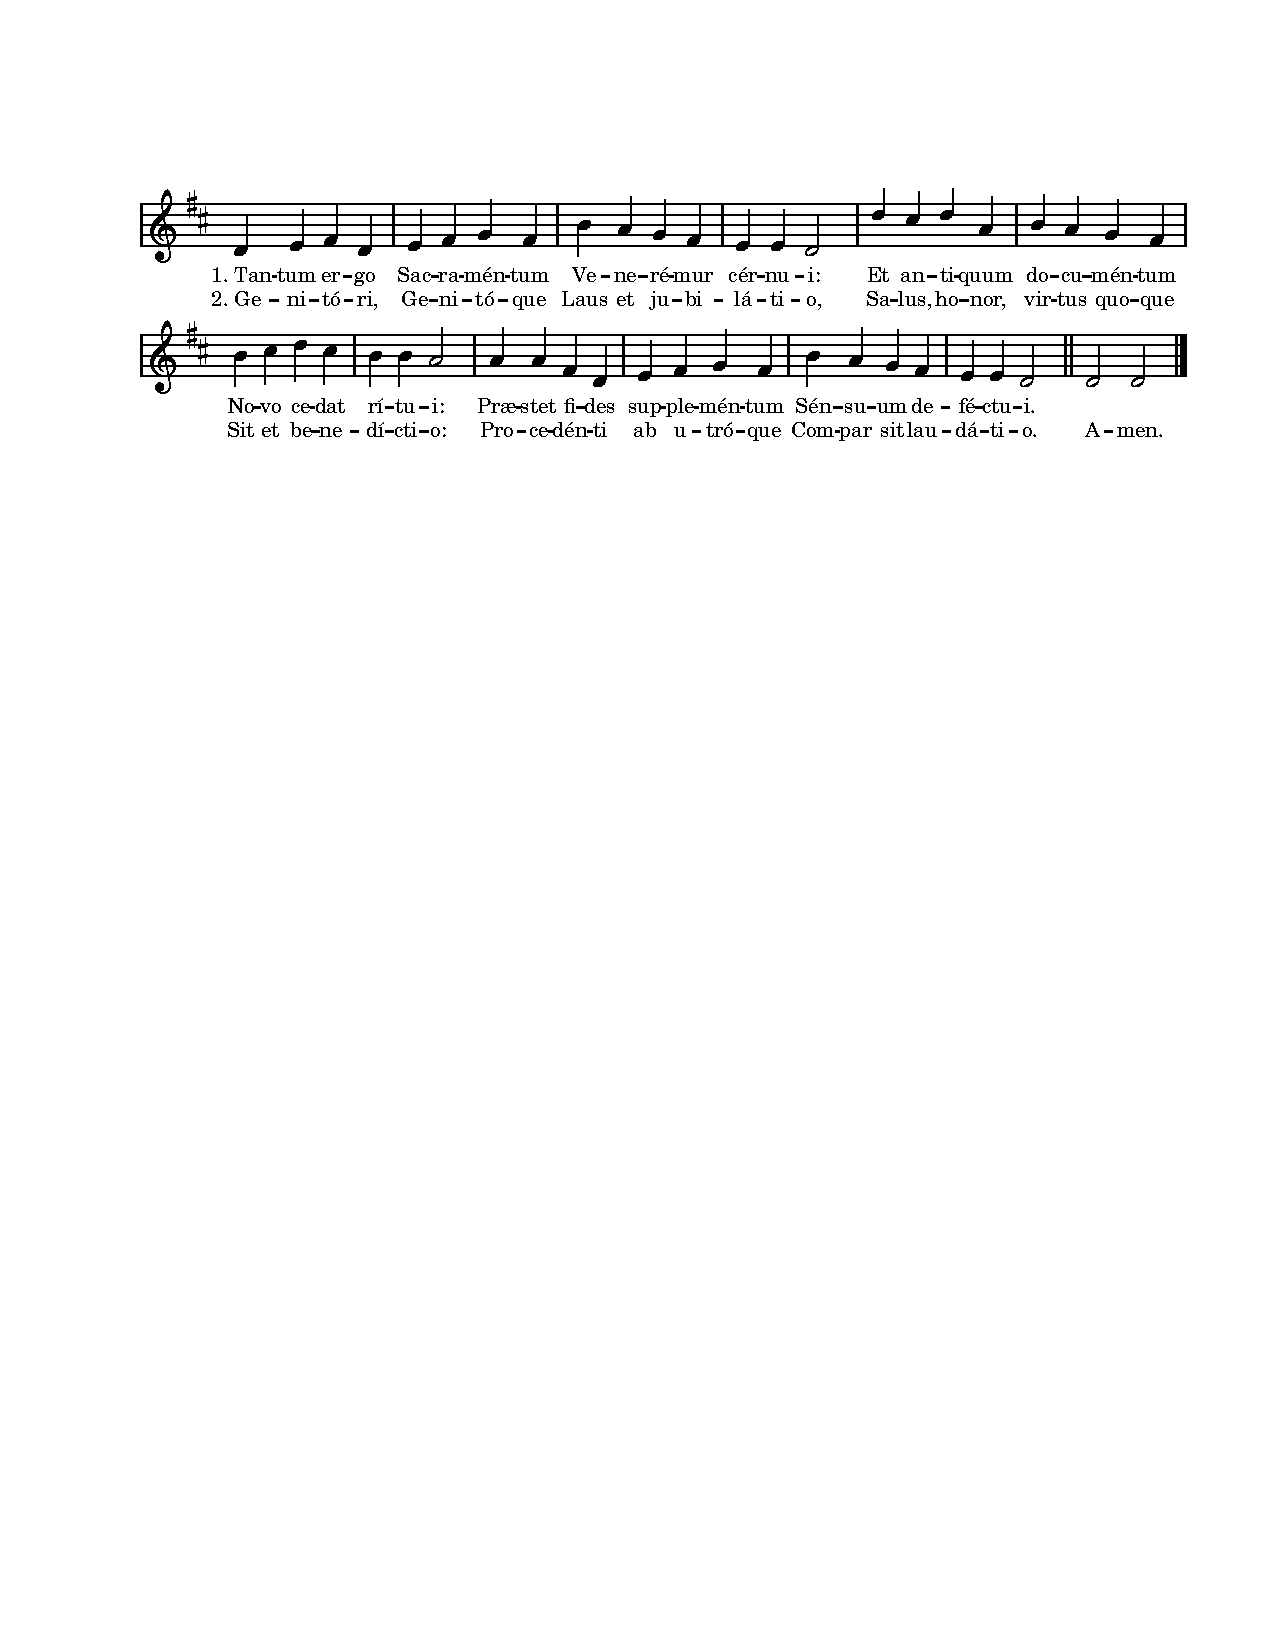
\includegraphics[scale=0.75,keepaspectratio]{Tantum_Ergo_Sacramentum_Wade_melody_cropped}\par}}

%\newpage
%
%\smalltitle{The Divine Praises.}
%
%\textes{laudes_divinae_en}
%
%\rubrique{These are sung alternating between the cantors and the whole congregation. All sing \normaltext{Fiat, Fiat} at the end.}
%
%\gscore[]{}{laudes_divinae_no_breaks}

\end{document}